\documentclass{ximera}

\author{Anna Davis} \title{MTH 140 Homework 2} 

\begin{document}

\begin{abstract}

\end{abstract}
\maketitle
 \textit{Certificate due: 8/31/2020 at 11:59 p.m.}
\begin{problem}\label{prob:140hom2prob1}
The following table lists results of a survey of individuals with short commute times.
Find the relative frequency for each commute time interval.  Express relative frequency as a decimal (not a percent).  Round your answers to the nearest $100$th.
\begin{center}
\begin{tabular}{|c|c|c|}
 \hline
 &&   \\
 Commute Time (t)&Frequency& Relative Frequency \\
 &&   \\
  \hline
  &&  \\
 $0<t\leq 5$&$4180$&$\answer[tolerance=0.001]{0.074}$ \\
  && \\
 \hline
  && \\
 $5<t\leq 10$&$13687$&$\answer[tolerance=0.001]{0.244}$ \\
  && \\
 \hline
  && \\
  $10<t\leq 15$&$18618$&$\answer[tolerance=0.001]{0.332}$  \\
  && \\
 \hline
 && \\
  $15<t\leq 20$&$19634$&$\answer[tolerance=0.001]{0.35}$  \\
  && \\
 \hline
 \end{tabular}
\end{center}    
Data based on \href{https://en.wikipedia.org/wiki/Histogram}{https://en.wikipedia.org/wiki/Histogram}.
\end{problem}

\begin{problem}\label{prob:140hom2prob2}
Identify the type of graphical representation.
\begin{enumerate}
    \item Graphical Representation: \wordChoice{\choice{Histogram}, \choice[correct]{Bar Graph},\choice{Box Plot},\choice{Time Series},\choice{Stem-and-Leaf Plot}}
    \begin{image}
   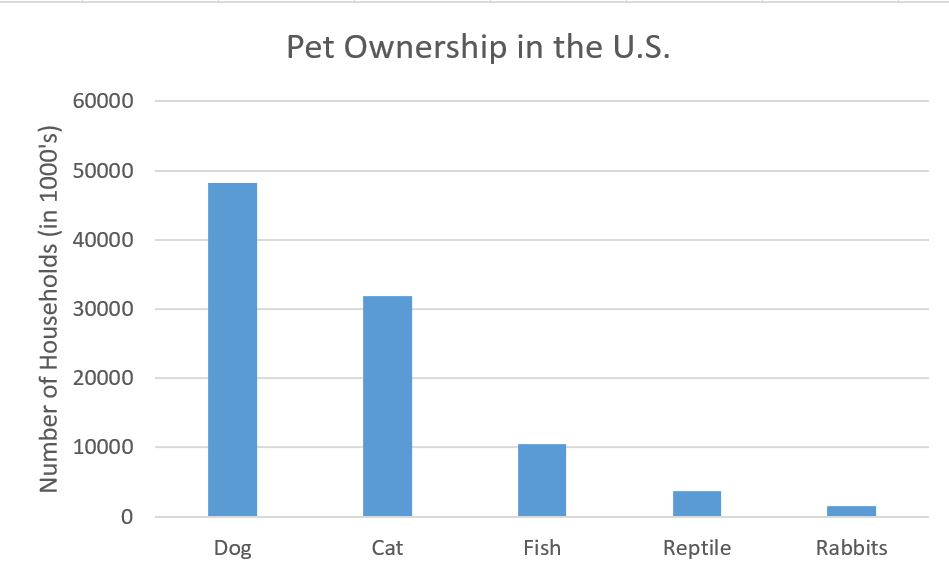
\includegraphics[height=1in]{140H2pic4.jpg}
 \end{image}
 
 Source: \href{https://www.avma.org/resources-tools/reports-statistics/us-pet-ownership-statistics}{https://www.avma.org/resources-tools/reports-statistics/us-pet-ownership-statistics}
 \item Graphical Representation: \wordChoice{\choice[correct]{Histogram}, \choice{Bar Graph},\choice{Box Plot},\choice{Time Series},\choice{Stem-and-Leaf Plot}}
    \begin{image}
   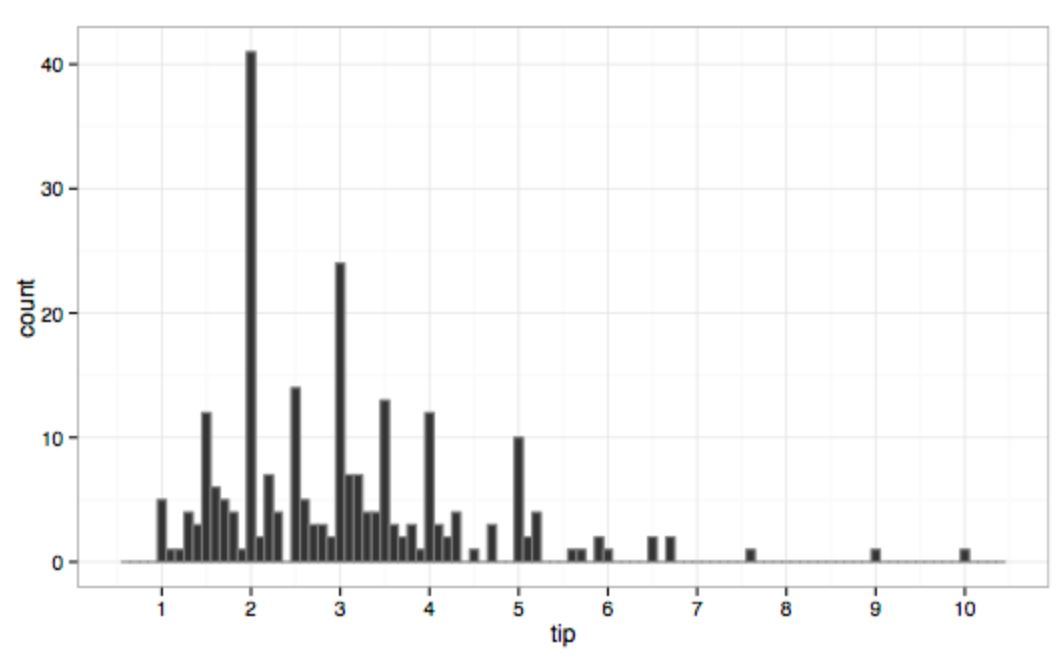
\includegraphics[height=1in]{140H2pic5.jpg}
 \end{image}
 Credit: Visnut / CC BY-SA (https://creativecommons.org/licenses/by-sa/4.0)
 \item Graphical Representation: \wordChoice{\choice{Histogram}, \choice{Bar Graph},\choice{Box Plot},\choice[correct]{Time Series},\choice{Stem-and-Leaf Plot}}
    \begin{image}
   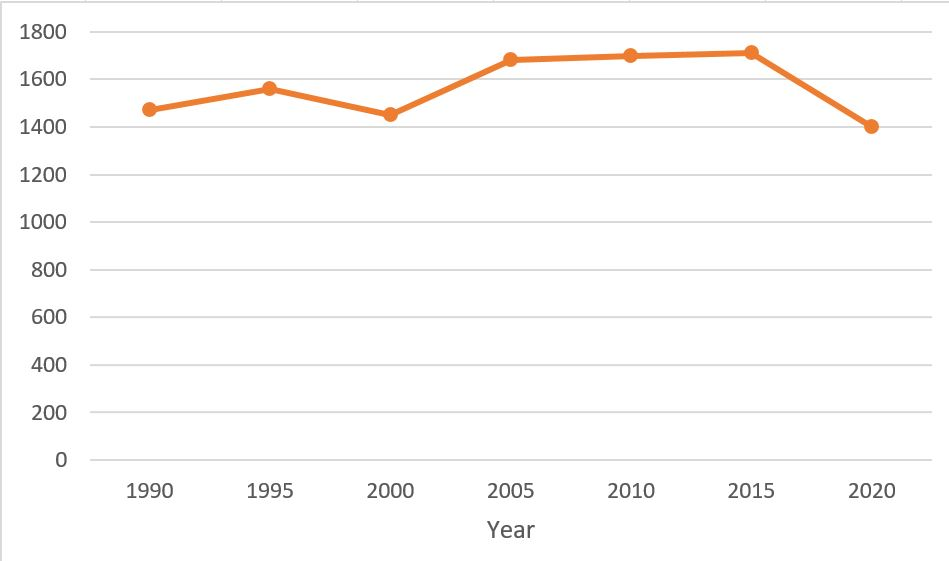
\includegraphics[height=1in]{140H2pic2.jpg}
 \end{image}
 \item Graphical Representation: \wordChoice{\choice{Histogram}, \choice{Bar Graph},\choice{Box Plot},\choice{Time Series},\choice[correct]{Stem-and-Leaf Plot}}
    \begin{image}
   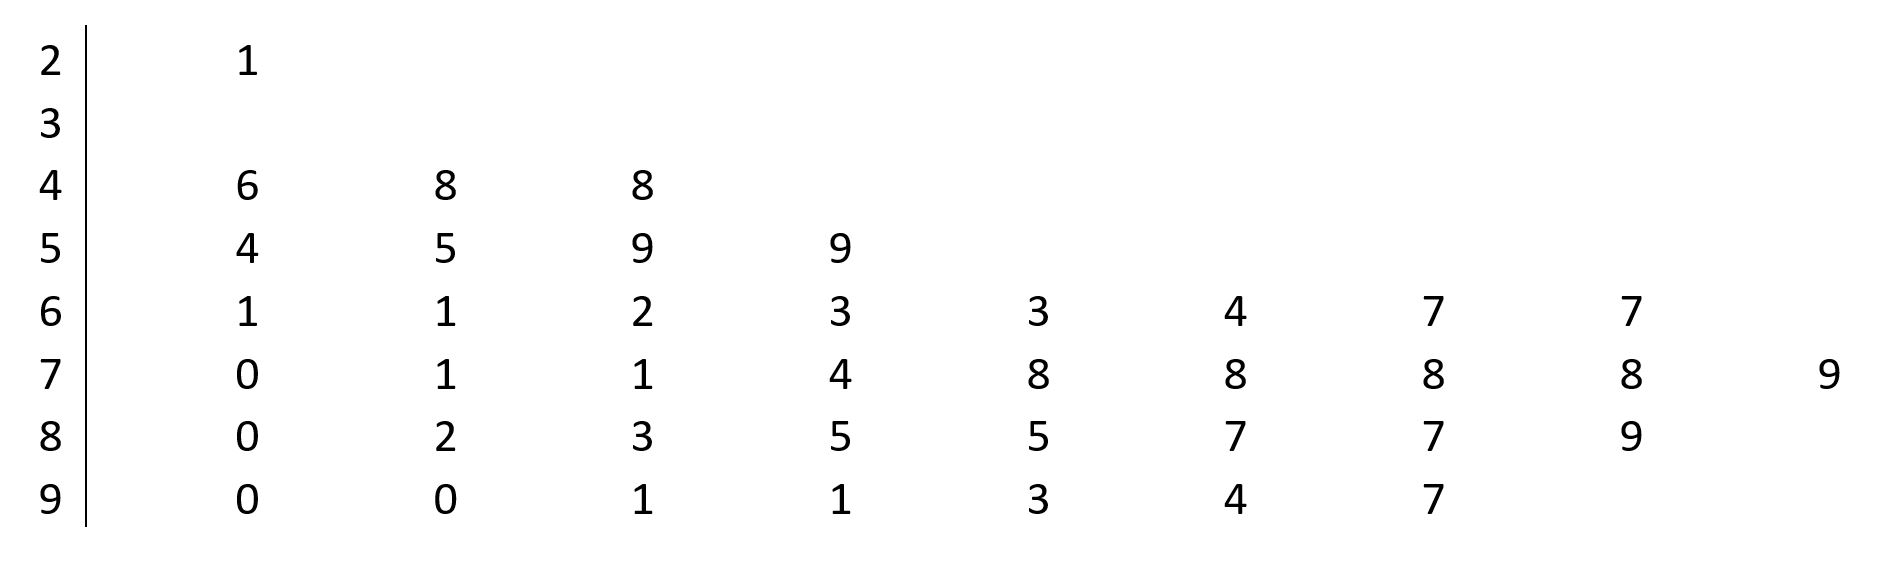
\includegraphics[height=1in]{140H2pic1.jpg}
 \end{image}
 \item Graphical Representation: \wordChoice{\choice{Histogram}, \choice{Bar Graph},\choice[correct]{Box Plot},\choice{Time Series},\choice{Stem-and-Leaf Plot}}
    \begin{image}
   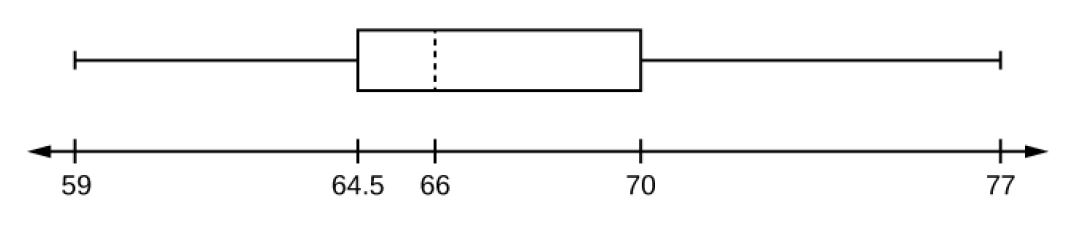
\includegraphics[height=1in]{140H2pic3.jpg}
 \end{image}
 Source: \href{https://openstax.org/details/books/introductory-statistics}{https://openstax.org/details/books/introductory-statistics} p. 97.
\end{enumerate}
\end{problem}

\begin{problem}\label{prob:140hom2prob3}
The histogram below shows the number of absences that occurred over one semester period in Mrs. Miller's fifth grade class.  For example, this graph tells us that the number of students incurring 2 absences is 5.

\begin{image}
   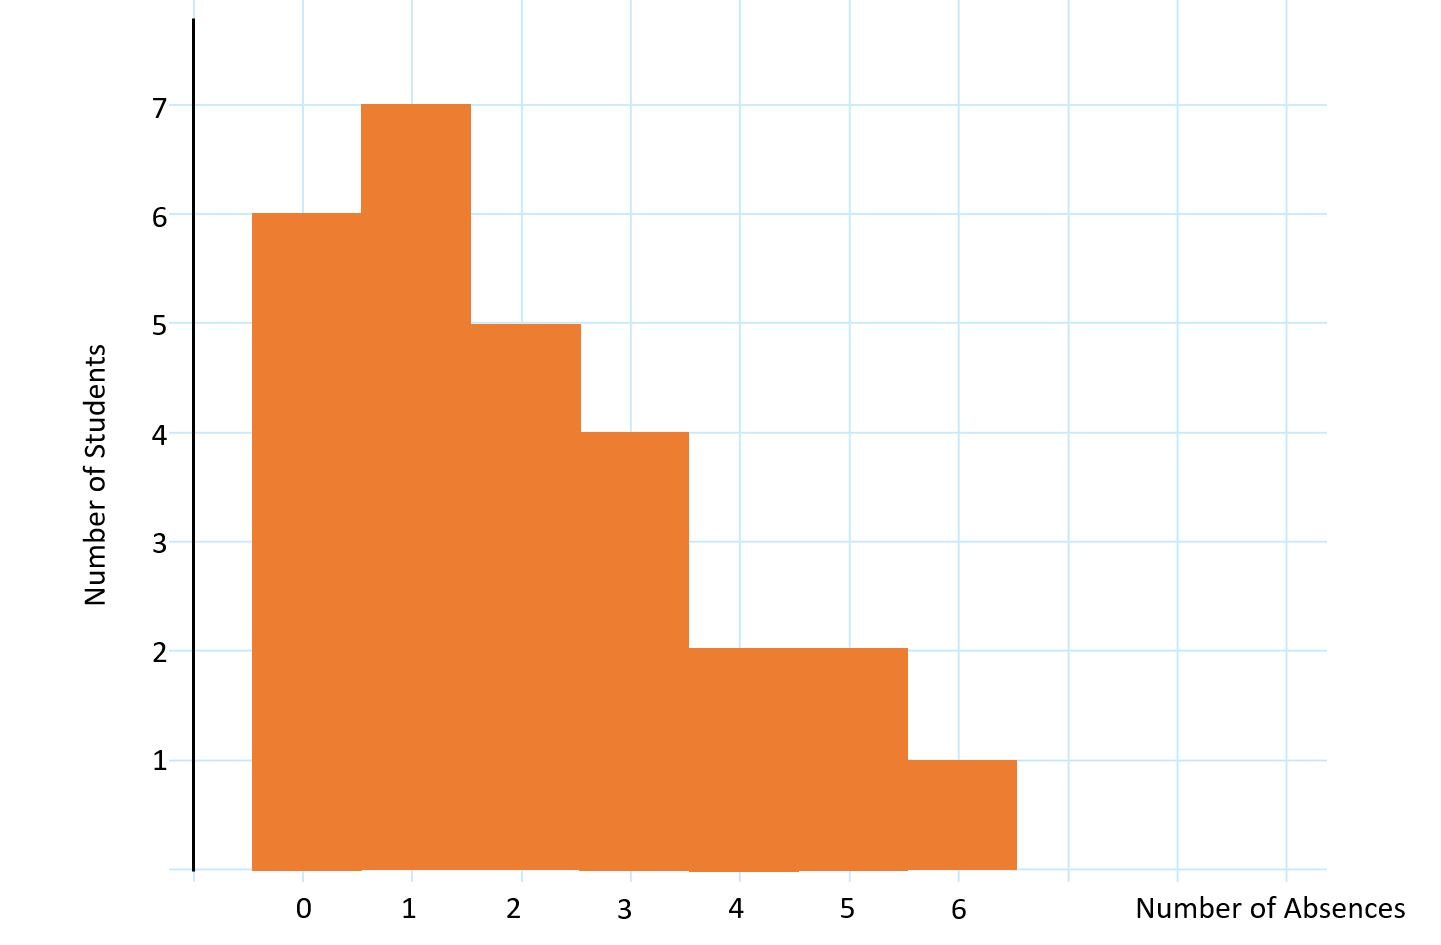
\includegraphics[height=1in]{140H2pic6.jpg}
 \end{image}
 
 Use the graph to answer the following questions.
 
 \begin{enumerate}
     \item How many students incurred 3 absences? $\answer{4}$
     \item What is the mode? $\answer{1}$
     \item How many students are in the class? $\answer{27}$
     \item What is the mean number of absences? $\answer[tolerance=0.01]{1.96}$
     \item What is the median number of absences? $\answer{2}$
 \end{enumerate}
\end{problem}

\begin{problem}\label{prob:140hom2prob4}
The following is a summary test results for an introductory History course.
\begin{image}
   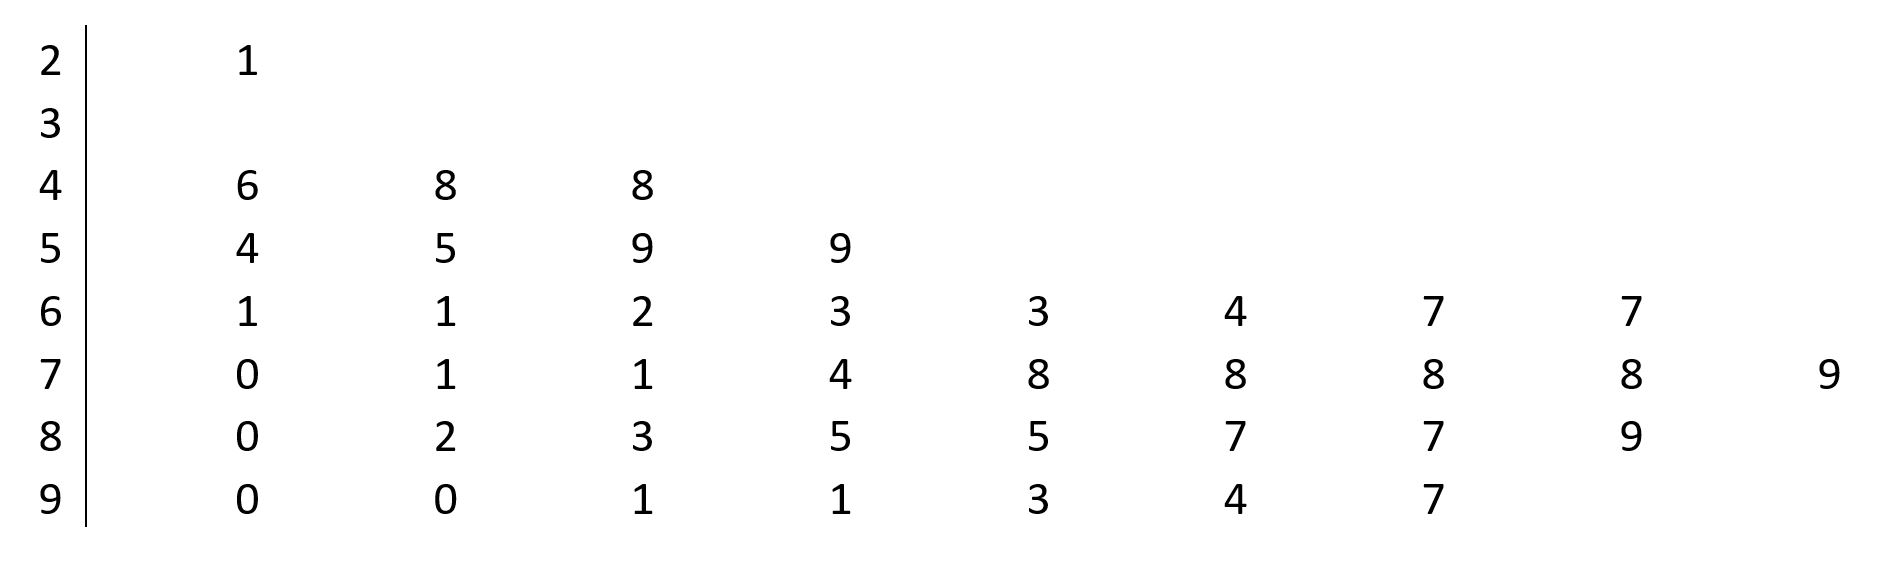
\includegraphics[height=1in]{140H2pic1.jpg}
 \end{image}
 
 Use this information to answer the following questions.
 
 \begin{enumerate}
     \item How many students took the class? $\answer{41}$
     \item What is the mode? $\answer{78}$
     \item What is the median score? $\answer{78}$
     \item $Q1=\answer{61.5}$
     \item $Q3=\answer{87}$
     \item $\mbox{IQR}=\answer{25.5}$
     \item Outlier Score(s): $\answer{21}$
     \item 20 th percentile is $\answer{60}$
     \item 60 th percentile is $\answer{79.5}$
     \item 80 th percentile is $\answer{89}$
 \end{enumerate}
\end{problem}


\end{document} 


